\section{Introduction}
\label{sec:introduction}
Generating collision-free trajectories when dealing with multiagent systems is a safety-critical task. In missions that require cooperation of multiple agents, such as warehouse management \cite{guizzo2008three}, it is often desirable to safely drive the agents from a starting location to a final location. Solving this problem, known as multiagent point-to-point transitions, is therefore an integral objective of any robust multiagent system.

There are two main variations of the multiagent point-to-point transition problem: the labelled or the unlabelled agent problems. In the former, each agent has a fixed final position that cannot be exchanged with other agents \cite{schouwenaars2001mixed, augugliaro2012generation}; in the latter, the algorithm is free to assign the goals to the agents, as to ease the complexity of the trajectories \cite{turpin2012decentralized}. This paper will focus on the labelled agent version of the problem. 

A natural way to formulate the problem is as an optimization problem. One of the first approaches proposed the use if Mixed Integer Linear Programming (MILP), modelling collision constraints as binary variables \cite{schouwenaars2001mixed}. These methods, although viable, are computationally heavy and not suited for large teams.

More recently, techniques based on Sequential Convex Programming (SCP) \cite{boyd2008sequential}  proved to improve the computational tractability of the algorithms. In \cite{augugliaro2012generation}, SCP is used to solve the optimal-fuel trajectories of quadrotor teams midflight. A decoupled version of that algorithm (dec-iSCP) is proposed in \cite{chen2015decoupled}, which has shorter computation time at the cost of suboptimal solutions. As later seen in Sec bla bla, even in the decoupled formulation, computation time and feasibility of the problem does not scale well with the number of agents, primarily because the problem itself is harder to solve. 

A new solution to the problem is proposed in this paper, based on distributed model predictive control (DMPC) \cite{camponogara2002distributed}. Synchronous implementation of DMPC \cite{dai2017distributed}, allows the agents to solve their optimization problem in parallel, which significantly reduces computation time with respect to previous methods. Previous work on DMPC show its capabilities in multiagent tasks, such as formation control \cite{van2017distributed,turpin2012decentralized}, but not explicitly for point-to-point transitions. Moreover, the prediction horizon enables the agents to foresee future collisions and replan their trajectories, making the algorithm robust to infeasibility issues in previous decoupled techniques such as dec-iSCP.

\begin{figure}[t]
	\centering
	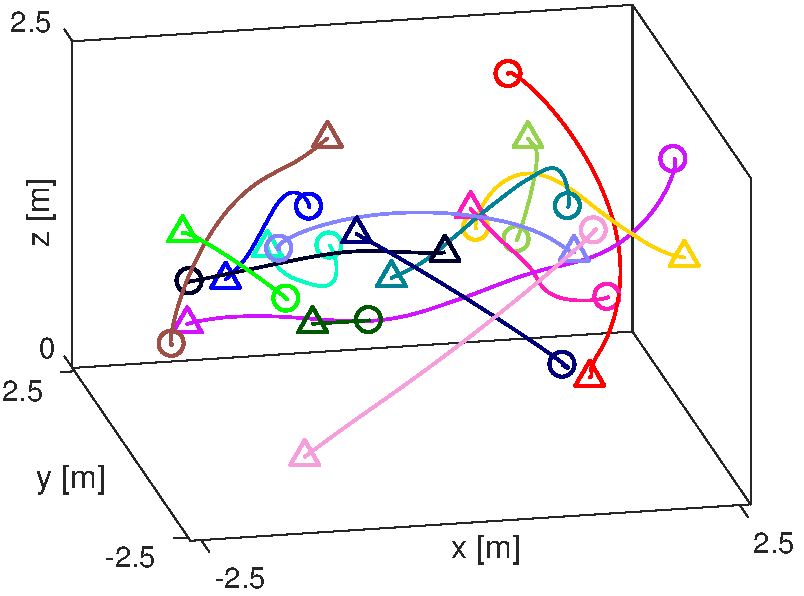
\includegraphics[width=0.45\textwidth]{figures/30_rand}
	\caption{A 25-vehicle point-to-point transition solved using our DMPC algorithm. The initial and final positions were chosen randomly within a convex volume of $5 \times 5 \times 2$ m. The agents were required to maintain a minimum distance of 0.75m of each other throughout the whole trajectory. Even in this highly cluttered dynamic environment, the proposed algorithm is capable of quickly finding a collision-free trajectory for all agents.}
	\label{fig:30_random}
\end{figure}

ieurgeruigher





